\section{Trigonometry}
\begin{outline}

\0
\subsection{Trigonometric ratios}
	\1 What is trigonometry?
		\2 Trigonometry is the study of the relationship between the angles and side lengths of triangles. It is built upon three ratios: sine, cosine, and tangent. A common mnemonic is SOHCAHTOA, for remembering the trigonometric ratios, with S representing sine, C representing cosine, and T representing tangent. Respectively, O, A, and H mean opposite, adjacent, and hypotenuse.
		
\begin{center}
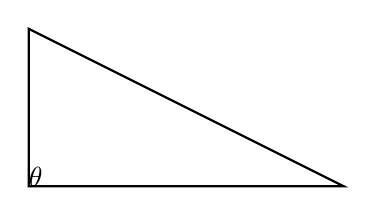
\begin{tikzpicture}[thick]
\coordinate (O) at (0,0);
\coordinate (A) at (4,0);
\coordinate (B) at (0,2);
\draw (O)--(A)--(B)--cycle;

\tkzLabelSegment[below=2pt](O,A){\textit{adjacent}}
\tkzLabelSegment[left=2pt](O,B){\textit{opposite}}
\tkzLabelSegment[above right=2pt](A,B){\textit{hypotenuse}}

\tkzMarkRightAngle[fill=white,size=0.5,opacity=.4](A,O,B)
\tkzLabelAngle[pos = 0.35](A,O,B){}

\tkzMarkAngle[fill= white,size=1.2cm,%
opacity=.4](B,A,O)
\tkzLabelAngle[pos = 0.9](B,A,O){$\theta$}

\tkzMarkAngle[fill= white,size=0.7cm,%
opacity=.4](O,B,A)
\tkzLabelAngle[pos = 0.5](O,B,A){}

\end{tikzpicture}
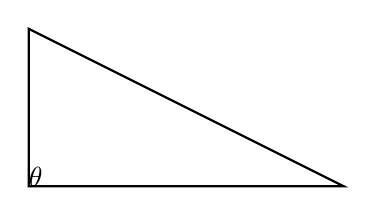
\begin{tikzpicture}[thick]
\coordinate (O) at (0,0);
\coordinate (A) at (4,0);
\coordinate (B) at (0,2);
\draw (O)--(A)--(B)--cycle;

\tkzLabelSegment[below=2pt](O,A){\textit{opposite}}
\tkzLabelSegment[left=2pt](O,B){\textit{adjacent}}
\tkzLabelSegment[above right=2pt](A,B){\textit{hypotenuse}}

\tkzMarkRightAngle[fill=white,size=0.5,opacity=.4](A,O,B)
\tkzLabelAngle[pos = 0.35](A,O,B){}

\tkzMarkAngle[fill= white,size=1.2cm,%
opacity=.4](B,A,O)
\tkzLabelAngle[pos = 0.9](B,A,O){}

\tkzMarkAngle[fill= white,size=0.7cm,%
opacity=.4](O,B,A)
\tkzLabelAngle[pos = 0.5](O,B,A){$\theta$}

\end{tikzpicture}
\end{center}

	\1 The three trigonometric ratios
		\2 Sine of angle $\theta$ (\textbf{sin} $\theta$)
			\3 ``SOH''
				\[\sin{\theta} = \frac{opposite}{hypotenuse}\]
		\2 Cosine of angle $\theta$ (\textbf{cos} $\theta$)
			\3 ``CAH''
				\[\sin{\theta} = \frac{adjacent}{hypotenuse}\]
		\2 Tangent of angle $\theta$ (\textbf{tan} $\theta$)
			\3 ``TOA''
				\[\sin{\theta} = \frac{opposite}{adjacent}\]

	\1 Finding an unknown numerator
		\2 Finding an unknown numerator involves multiplying the entire equation by the denominator, and then calculating the result.
			\3 Example -- Finding an unknown numerator
				\[\sin \theta = \frac{O}{H}\]
				\[\sin 30\degree = \frac{x}{10}\]
				\[\therefore x = 10 \times \sin 30\degree \]
				\[= 5\]
	\1 Finding an unknown denominator
		\2 Finding an unknown denominator involves multiplying the entire equation by the denominator, then dividing the entire equation by the $\sin\theta$ expression. Once that has been done, the result is easily calculated.
			\3 Example -- Finding an unknown denominator
				\[\sin\theta = \frac{O}{H}\]
				\[\sin 30\degree = \frac{10}{x}\]
				\[x \times \sin 33\degree = 10\]
				\[x = \frac{10}{\sin 30\degree}\]
				\[= 20\]

\0
\subsection{Finding angles}
	\1 Inverse trigonometric functions
		\2 $\sin$, $\cos$, and $\tan$ are not only used for finding side lengths. They can also be used as inverse trigonometric functions. The inverse function is shown as $sin^{-1}$, $cos^{-1}$, or $tan^{-1}$. Inverse trigonometric (trig for short) functions are able to find angles from the side lengths.
			\3 Example -- Inverse trigonometric functions
				\[\sin\theta = \frac{1}{2}\]
				\[\therefore \theta = \sin^{-1}\bigg(\frac{1}{2}\bigg)\]
				\[= 30\degree\]

\0
\subsection{Applications in two dimensions}
	\1 Angle of elevation
		\2 Angle of elevation refers to an angle raising higher than horizontal. Hence, it is measured \textit{up} from the horizontal.
	\1 Angle of depression
		\2 Angle of depression refers to an angle dropping lower than horizontal. Hence, it is measured \textit{down} from the horizontal.

\0
\subsection{Bearings}
	\1 True bearings
		\2 Bearings are the use of degrees as a directional reference point. They are important in navigation, and have a very important value in real world application.
	\1 Use in trigonometry
		\2 Use of bearings in trigonometry is very simple. With $0\degree$ as North, $90\degree$ as East, $180\degree$ as South, and $270\degree$ as West, exact directions and distances are able to be found using trigonometric functions involving the fixed reference lines created by the North to South, and West to East directions.

\0
\subsection{Applications in three dimensions}
	\1 2D vs 3D trigonometry
		\2 Although right-angled triangles are 2D shapes, they still hold value in three dimensions. Trigonometry in 3D is identical to trigonometry in 2D. There are just more things to consider. Firstly, 3D trigonometry involves visualisation and rendering 3D into 2D triangles. Next, it is essential to use the trigonometric ratios to find unknowns that will allow a greater control over what calculations can be computed. Lastly, perhaps the most important part of applying trigonometry to 3 dimensions is relating the answers from two-dimensions back to the original object.

\0
\subsection{Obtuse angles and exact values}
	\1 The unit circle
		\2 The unit circle is a circle with a radius of 1 unit. It is used to define $\sin\theta$, $\cos\theta$, and $\tan\theta$ for all angles $\theta$. A point $P(x, y)$ is a point on the unit circle defined by an angle $\theta$ measured anticlockwise from the positive $x$-axis $(1, 0)$.
\begin{center}
\begin{tikzpicture}[scale=2.5,cap=round,>=latex]
        \draw[->] (-1.5cm,0cm) -- (1.5cm,0cm) node[right,fill=white] {$x$};
        \draw[->] (0cm,-1.5cm) -- (0cm,1.5cm) node[above,fill=white] {$y$};
        \coordinate (O) at (0cm,0cm);
        \coordinate (A) at (0.7071cm,0cm);
        \coordinate (B) at (0.7071cm,0.7071cm);
        \draw[dashed] (O)--(A)--(B)--cycle;
        \tkzLabelSegment[above left=-3pt](O,B){\textit{$1$}}
        \tkzMarkRightAngle[fill=white,size=0.15,opacity=0.5](B,A,O)
        \tkzLabelAngle[pos = 0.35](B,A,O){}
        
        \tkzMarkAngle[fill= white,size=0.2cm,opacity=1](A,O,B)
        \tkzLabelAngle[pos = 0.14](A,O,B){$\theta$}

        \draw[thick] (0cm,0cm) circle(1cm);

        \foreach \x in {0,90,180,270,360} {
                \draw[gray] (0cm,0cm) -- (\x:1cm);
                \filldraw[black] (\x:1cm) circle(0.4pt);
        }
        \foreach \x in {
            30,
            45,
            60,
            90,
            120,
            135,
            150,
            180,
            210,
            225,
            240,
            270,
            300,
            315,
            330,
            360}
                \draw (\x:0.85cm) node[] {};
        \foreach \x/\xtext/\y in {
            30/\frac{\sqrt{3}}{2}/\frac{1}{2},
            45/\frac{\sqrt{2}}{2}/\frac{\sqrt{2}}{2},
            60/\frac{1}{2}/\frac{\sqrt{3}}{2},
            150/-\frac{\sqrt{3}}{2}/\frac{1}{2},
            135/-\frac{\sqrt{2}}{2}/\frac{\sqrt{2}}{2},
            120/-\frac{1}{2}/\frac{\sqrt{3}}{2},
            210/-\frac{\sqrt{3}}{2}/-\frac{1}{2},
            225/-\frac{\sqrt{2}}{2}/-\frac{\sqrt{2}}{2},
            240/-\frac{1}{2}/-\frac{\sqrt{3}}{2},
            330/\frac{\sqrt{3}}{2}/-\frac{1}{2},
            315/\frac{\sqrt{2}}{2}/-\frac{\sqrt{2}}{2},
            300/\frac{1}{2}/-\frac{\sqrt{3}}{2}}
                \draw (\x:1.25cm) node[fill=white] {};
        \draw (-1.25cm,0cm) node[fill=white] {$-1$}
              (1.25cm,0cm)  node[fill=white] {$1$}
              (0cm,-1.25cm) node[fill=white] {$-1$}
              (0cm,1.25cm)  node[fill=white] {$1$};
        \draw (0cm,0cm) -- (0.7071cm,0.7071cm);
    \end{tikzpicture}
    \end{center}
	\1 Two special triangles
		\2 There are two special triangles used in trigonometry, which allow one to easily find exact values for $\sin\theta$, $\cos\theta$, and $\tan\theta$. Pythagoras theorem can trivially be used to confirm the length of each side.

\begin{center}
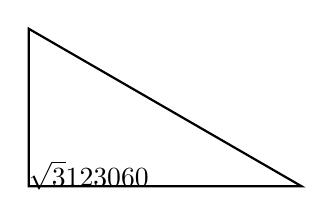
\begin{tikzpicture}[thick]
\coordinate (O) at (0,0);
\coordinate (A) at (3.4641,0);
\coordinate (B) at (0,2);
\draw (O)--(A)--(B)--cycle;
\tkzLabelSegment[below=1.5pt](O,A){\textit{$\sqrt{3}$}}
\tkzLabelSegment[left=1.5pt](O,B){\textit{$1$}}
\tkzLabelSegment[above right=1.5pt](A,B){\textit{$2$}}
\tkzMarkRightAngle[fill=white,size=0.5,opacity=.4](A,O,B)
\tkzLabelAngle[pos = 0.35](A,O,B){}
\tkzMarkAngle[fill= white,size=1.3cm,
opacity=.4](B,A,O)
\tkzLabelAngle[pos = 0.95](B,A,O){$30\degree$}
\tkzMarkAngle[fill= white,size=0.9cm,%
opacity=.4](O,B,A)
\tkzLabelAngle[pos = 0.7](O,B,A){$60\degree$}
\end{tikzpicture}
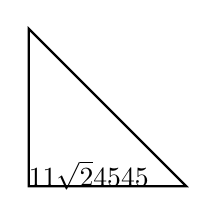
\begin{tikzpicture}[thick]
\coordinate (O) at (0,0);
\coordinate (A) at (2,0);
\coordinate (B) at (0,2);
\draw (O)--(A)--(B)--cycle;
\tkzLabelSegment[below=1.5pt](O,A){\textit{$1$}}
\tkzLabelSegment[left=1.5pt](O,B){\textit{$1$}}
\tkzLabelSegment[above right=1.5pt](A,B){\textit{$\sqrt{2}$}}
\tkzMarkRightAngle[fill=white,size=0.5,opacity=.4](A,O,B)
\tkzLabelAngle[pos = 0.35](A,O,B){}
\tkzMarkAngle[fill= white,size=1cm,%
opacity=.4](B,A,O)
\tkzLabelAngle[pos = 0.7](B,A,O){$45\degree$}
\tkzMarkAngle[fill= white,size=1cm,%
opacity=.4](O,B,A)
\tkzLabelAngle[pos = 0.8](O,B,A){$45\degree$}
\end{tikzpicture}
\end{center}

\0
\subsection{The sine rule}
	\1 Finding the sine rule

\begin{center}
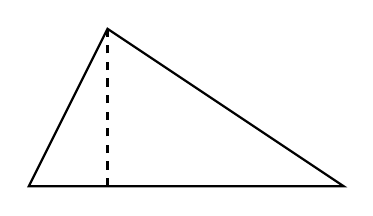
\begin{tikzpicture}[thick]
\coordinate (A) at (0,0);
\coordinate (B) at (4,0);
\coordinate (C) at (1,2);
\coordinate (P) at (1,0);
\draw (B)--(A)--(C)--cycle;
\draw [dashed] (P)--(C);

\tkzLabelSegment[below=2pt](A,B){\textit{c}}
\tkzLabelSegment[left=2pt](A,C){\textit{b}}
\tkzLabelSegment[above right=2pt](B,C){\textit{a}}
\tkzLabelSegment[right=2pt](P,C){\textit{h}}
\tkzLabelPoint[above=2pt](C){\textit{C}}
\tkzLabelPoint[below left=2pt](A){\textit{A}}
\tkzLabelPoint[below right=2pt](B){\textit{B}}
\tkzLabelPoint[below=2pt](P){\textit{P}}
\tkzMarkAngle[fill= white,size=0.6cm,%
opacity=.4](B,A,C)
\tkzMarkAngle[fill= white,size=0.5cm,%
opacity=.4](A,C,B)
\tkzMarkAngle[fill= white,size=0.8cm,%
opacity=.4](C,B,A)
\end{tikzpicture}
\end{center}
		\[\text{From }\Delta \text{CPB} \text{, } \frac{h}{a} = \text{sin } B\]
		\[\text{so\ \ \ \ \ \ \ \ } h = a \text{ sin } B\]
		\[\text{From }\Delta \text{CPA} \text{, } \frac{h}{b} = \text{sin } A\]
		\[\text{so\ \ \ \ \ \ \ \ } h = b \text{ sin } A\]
		\[\therefore a \text{ sin } B = b \text{ sin } A \text{\ \ or\ \ } \frac{a}{\text{sin } A} = \frac{b}{\text{sin } B}\]
		\[\text{Similarly:\ \ } \frac{a}{\text{sin } A} = \frac{c}{\text{sin } C} \text{\ \ and\ \ } \frac{b}{\text{sin } B} = \frac{c}{\text{sin } C}\]
		\2 When using the sine rule, label triangles with capital letters for vertices and the corresponding lower case letter for the side opposite the angle.
		\2 The sine rule states that the ratios of each side of a triangle to the sine of the opposite angle are equal. The sine rule holds true for both acute- and obtuse-angled triangles.
			\3 Equation
				\[\frac{a}{\text{sin } A} = \frac{b}{\text{sin } B} = \frac{c}{\text{sin } C}\]
		\2 The ambiguous case arises when we are given two sides and an angle that is not the included angle. Calculation of the result will yield two results: an obtuse angle, and an acute angle. There will be only one result of the equation itself, however finding the supplementary angle of the result will find the obtuse given an acute, and vice versa. The choice of using an obtuse or an acute angle is based on whether $\theta$ in the equation is obtuse or acute.
	\1 Finding a side length using the sine rule
		\2 To find an unknown side length, one must find the correct sine rule relationship to apply in the situation. Finding the unknown is as simple as substituting in values to the sine rule relationship, and solving the equation.
	\1 Finding an angle using the sine rule
		\2 

\0
\subsection{The cosine rule}

\0
\subsection{Area of a triangle}

\0
\subsection{The four quadrants}

\0
\subsection{Graphs of trigonometric functions}

\end{outline}
